\section{Results}\label{sec:results}
In this section we will show the results of our analysis. First we will present some descriptive statistics on our data. In the second subsection the results of the paired $t$-test, including the rejection or the acceptance of our hypothesis is presented, and in the remainder there is some further analysis based on the data collected.

%\textcolor{red}{Provide:}
%\begin{itemize}
%\item \textcolor{red}{descriptive statistics}
%\item \textcolor{red}{hypothesis testing}
%\end{itemize}
%\textcolor{red}{Also, provide suitable graphs to illustrate your results.}
\subsection{Descriptive statistics}
\begin{table}[h]
    \centering
\begin{tabular}{|c|c|c|c|}
    \hline
    Application & Average (J) & Minimal (J) & Maximal (J)\\
    \hline
    Google Maps & 80.18 & 47.85 & 110.05 \\
    YouTube & 3.67& 0.48 & 10.09\\
    Facebook & 31.22 & 3.94 &  83.52\\
    Instagram & 8.82 & 4.62 & 14.35\\
    Twitter & 1.92 & 0.25 & 4.67\\
    \hline
    \end{tabular}
    \caption{Average, minimal and maximal energy consumption of running a scenario on native applications}
    \label{tab:native-datapoints}
\end{table}


After collecting the data, the data-set contains a meaningful number of metrics. In \autoref{tab:native-datapoints} we see for each native mobile app the average energy consumption per run, the energy consumption of the run with the least energy consumption and the energy consumption of the run with the largest energy consumption. The same metrics are presented for the mobile web applications in \autoref{tab:web-datapoints}. The difference for each application is presented in \autoref{tab:differences}.

In these basic metrics we can already see some differences between the energy consumption between native mobile applications and mobile web applications. We also see that some applications use way more energy than others (i.e. Google Maps maximally consumes 110.05J on mobile phone, while Twitter only maximally consumes 4.67J on the same device), but also that some applications use more energy as mobile web application than as native mobile application (i.e. Instagram's average energy consumption of running a scenario on web application is 13.36J which is higher than on native application 8.82J), while others use more energy when run as native mobile application than as mobile web application (i.e. Instagram's minimal energy consumption of running a scenario on native application is 4.62J which is higher than on web application 1.90J).

\begin{table}[h]
    \centering
\begin{tabular}{|c|c|c|c|}
    \hline
    Application & Average (J)& Minimal (J)& Maximal (J)\\
    \hline
    Google Maps & 3.85 & 0.35 & 11.76 \\
    YouTube & 2.44 & 0.30 & 8.37 \\
    Facebook & 48.28 & 35.33 & 60.00\\
    Instagram & 13.36 & 1.90 & 35.71 \\
    Twitter & 2.36 & 0.75 & 6.56\\
    \hline
    \end{tabular}
    \caption{Average, minimal and maximal energy consumption of running a scenario on web applications}
    \label{tab:web-datapoints}
\end{table}

\begin{table}[h]
    \centering
\begin{tabular}{|c|c|c|c|}
    \hline
    Application & Difference (native - web) (J) \\
    \hline
    Google Maps & 76.33 \\
    YouTube & 1.23 \\
    Facebook & -17.06  \\
    Instagram & -4.54 \\
    Twitter & -0.44  \\
    \hline
    \end{tabular}
    \caption{Differences in energy consumptions per application}
    \label{tab:differences}
\end{table}

\begin{figure*}[bt]
    \centering
    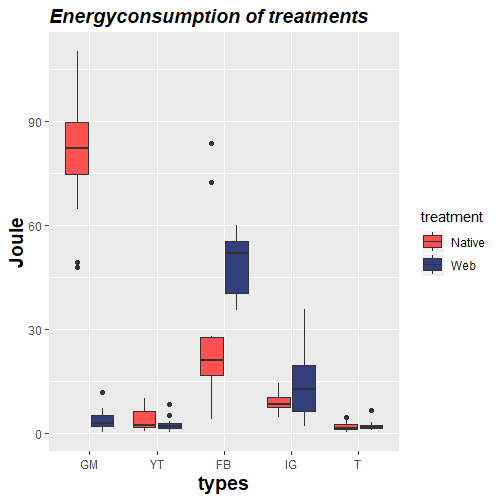
\includegraphics[width=0.5\textwidth]{AppVSweb/figures/Boxplots/Energyconsumption.png}
    \caption{Boxplots of the consumed energy per application}
    \label{fig:Econs}
\end{figure*}

The simple metrics presented in \autoref{tab:native-datapoints} and \ref{tab:web-datapoints} are just a very rough indication, which have to be refined with statistical analysis. In \autoref{fig:Econs} a set of boxplots showing the distribution of measurements for the runs of both the native mobile applications and the mobile web applications. These boxplots show the distribution of data per application, with the horizontal lines being the quartiles of the data, of which the middle one, the second quartile, is the median of the data. The whiskers range from the first and third quartile to the data extremes, as long as they are in 1.5 times the Inter Quartile Range, the outliers are the data points that do not fall within this range.

In this figure a trend is indicated that web applications use more energy than native applications, although not all applications follow this trend \textit{e.g.} YouTube and Google Maps, of which the latter is really deviant from the trend. However, this does not prove anything yet. To give some amount of certainty we need to perform a paired $t$-test if the assumptions for paired $t$-test are met, or a Wilcoxon signed-rank test if the assumptions for the paired $t$-test are not met.

To be able to perform a \textit{t}-test, we need to be certain that the data is in normally distributed. Because of the working of the paired \textit{t}-test, the data we care about are the differences between the pairs of applications. In \autoref{fig:diff_qq} there is a QQ-plot for these differences in energy consumption. This QQ-plot already gives an indication that the data is not normally distributed, as it does not follow a straight line.
% I know the QQ-plot maybe be irrelevant, but we still could use it. Then explain because we did not have time to test enough applications collecting enough data. So the result maybe irrelevant, is that ok?
% - We need a QQ-plot, but we need the right one. The ones already in the folder are probably irrelevant
\begin{figure}[t]
    \centering
    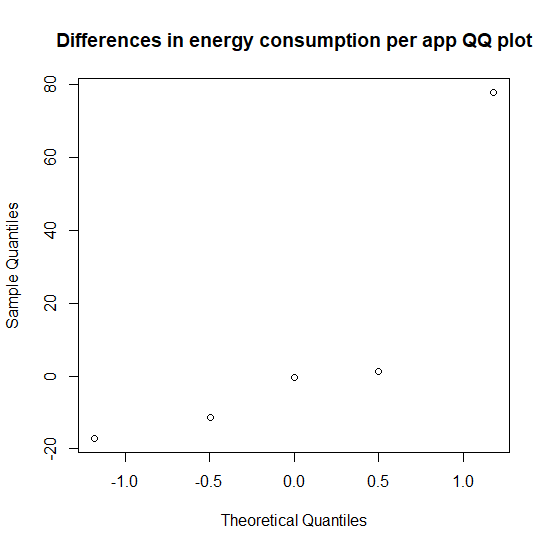
\includegraphics[width=\linewidth]{AppVSweb/figures/QQPlots/diff_qq.png}
    \caption{QQ plot for the differences in average energy consumption per application}
    \label{fig:diff_qq}
\end{figure}
Because the limited number of data-points, it is not obvious to determine whether or not the data is in normal distribution.

To get a more formal indication whether or not the data is normally distributed, a Shapiro-Wilk test for normality \cite{doi:10.1093/biomet/52.3-4.591} was performed on the data. This test returned a \textit{p-value} of 0.0189 for the `signed' differences between pairs, which is not within a 95\% confidence interval to accept normal distribution. When this set is converted to `unsigned' differences, this \textit{p-value} is still 0.01173, which doesn't fall in the 95\% confidence interval to accept the hypothesis that the data is normally distributed either. This means that to draw the right conclusions, we had to perform a non-parametric test on the data, in our case that is the Wilcoxon signed rank test \cite{10.2307/3001968}.


%To be very certain, a Shapiro-Wilk normality test was performed. These resulted in a \textit{p-value} (probability) of $3.3\times 10^{-8}$ for the web values, and $2.03\times10^{-12}$. This means that we need to reject the hypothesis that the data is in normal distribution. %NOTE: what does the data w/o the current Google Maps data? Because that data wildly differs from the other applications.
%\begin{figure}
%    \centering
%    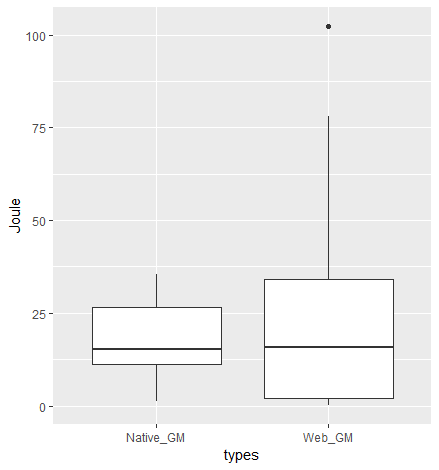
\includegraphics[width=\linewidth]{AppVSweb/figures/Boxplots/GooglemMaps_20.png}
%    \caption{Caption}
%    \label{fig:GMaps_boxplot}
%    %old version
%\end{figure}
% Title missing, need to be modified

%\begin{figure}
%    \centering
%    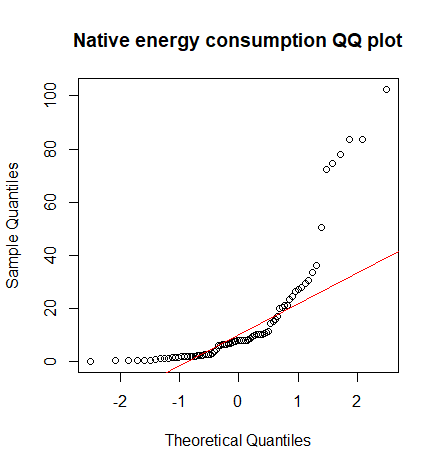
\includegraphics[width=\linewidth]{AppVSweb/figures/QQPlots/Native_energyconsumption_QQ.png}
%    \caption{QQPlot for the distribution for the energy consumption for native applications}
%    \label{fig:Dist2}
%\end{figure}

%\begin{figure}
%    \centering
%    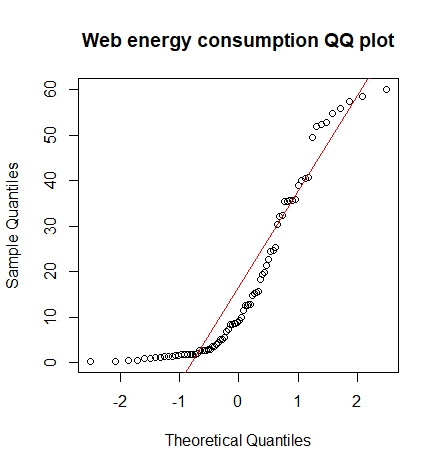
\includegraphics[width=\linewidth]{AppVSweb/figures/QQPlots/web_energyconsumption_QQ.png}
%    \caption{QQPlot for the distribution for the energy consumption for web applications}
%    \label{fig:Dist1}
%\end{figure}
%\begin{figure}
%    \centering
%    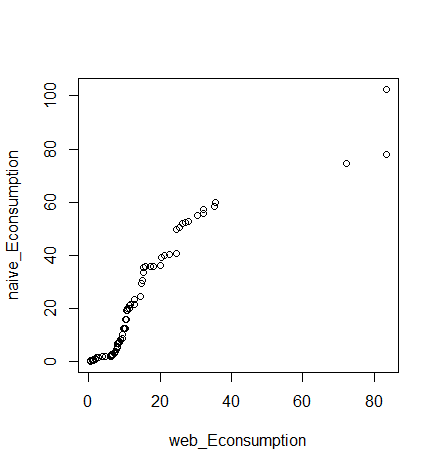
\includegraphics[width=\linewidth]{AppVSweb/figures/QQPlots/QQplot_joulevalues.png}
%    \caption{QQplot for the relative distribution of data}
%    \label{fig:joulevalues}
%\end{figure}


% CHeck for normality in distribution:

% Narmality test for data ( shapiro Wilk test) 
% native values:
% P = 3.27 * e^-8
% web values:
% P = 2.03 * e^-12
% If p < alpha (0.05) then it is NOT normally dist. 
 % + 
% see figures for QQ-plot 
%
\subsection{Hypothesis testing}
\textbf{RQ1} - How does energy efficiency ($\mathcal{E}$)  differ between native mobile applications and their mobile web counterparts?
\\
\newline 
The hypotheses for this research question were as follows:
\newline $H_0^1$        $\mathcal{E}_n = \mathcal{E}_w$ or in natural language: the energy consumption of native mobile applications is equal to the energy consumption of mobile web applications.
\newline $H_a^1$      $\mathcal{E}_n \neq \mathcal{E}_w$, the energy consumption of native mobile applications is not equal to the energy consumption of mobile web applications.

As was treated in the previous subsection, the data did not meet the requirements to perform a paired \textit{t}-test as the data was not in normal distribution. Because of this, the hypothesis was tested using the Wilcoxon signed rank test \cite{10.2307/3001968}. Unlike the t-test, the paired differences do not need to follow a normal distribution but the distribution of each side of the median - must have a similar shape. In other words the distribution of the differences must be symmetrical \cite{Wilcoxon}. Looking at \autoref{fig:LoGPlot} we assume it is quite symmetrical enough. 

\begin{figure}[t]
    \centering
    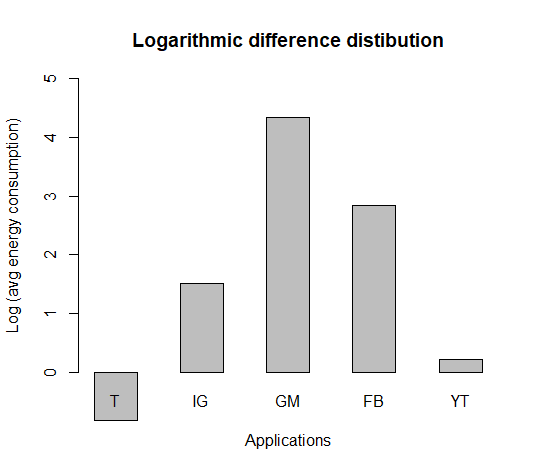
\includegraphics[width=\linewidth]{AppVSweb/figures/LoGPlot.png}
    \caption{Logarithmic distribution of the difference between treatments}
    \label{fig:LoGPlot}
\end{figure}


This test results in an p-value of 1 in an rejection of the null hypothesis that the energy consumption of native mobile applications is equal to the energy consumption of mobile web applications, and thus leads to the acceptance of the alternative hypothesis that the energy consumption of native mobile apps is not equal to the energy consumption of mobile web applications.
%shouldn't we remove the following part, as we didn't have time to dive into this?
\\\newline
Due to the small time-frame of this experiment, we did not have enough time to test our second research question. 

\subsection{Additional statistics}
\begin{figure}[ht]
    \centering
    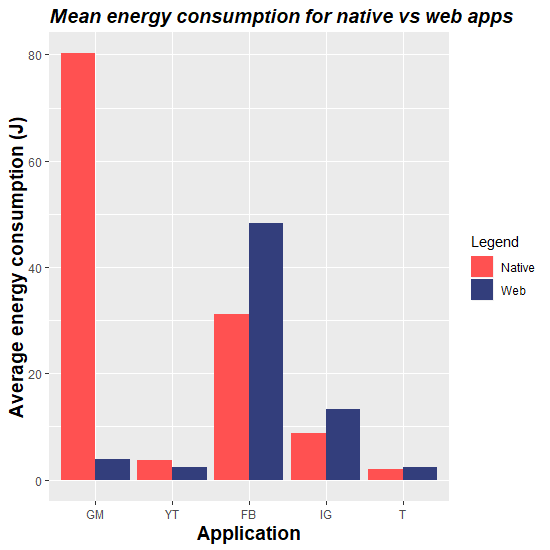
\includegraphics[width=\linewidth]{AppVSweb/figures/Barplot.png}
    \caption{Average energy consumption per application}
    \label{fig:bars}
\end{figure}
In \autoref{fig:bars} the average energy consumption of each application is shown, both as native mobile application as mobile web application. From this plot we see that the difference between native mobile applications and mobile web applications for some applications is limited, there are some applications that do have a significant difference between native mobile applications and mobile web applications. These applications usually have a more than average energy consumption for either native or web or both.

An interesting thing is that for example Google Maps does not only differ from the trend that mobile web applications use more energy than their native mobile counterparts, but does that with a very large difference, as the native mobile application does use quite a lot of energy, while the mobile web application does not use much more energy than for example the YouTube web application. 

A similar kind of result, but the other way around can be seen with the data from Facebook: both the native mobile application and the web application on average use more energy than most applications, but the mobile web application uses a lot more energy than the native mobile application.

Unfortunately, with the data that were collected for this paper it is almost impossible to find out why these differences happen. The reasons for these differences might be an interesting topic for a future research that is more focused on technical details and aimed at the perspective of software developers, but at this moment it goes way beyond the scope of this paper.
%\limit{Open - go deep as you wish}